% Finite-Element Implementation of a Hamilton-Principle Material Model for Oral Biofilms
% House format: Beamer Madrid / whale, aspectratio 169, STIX Two Text via fontspec.
% Build with xelatex (fontspec). See build.sh in this directory.
\documentclass[aspectratio=169,xcolor=dvipsnames]{beamer}

\usetheme{Madrid}
\usecolortheme{whale}

\usepackage{amsmath,amssymb}
\usepackage{fontspec}
\setmainfont[
  Path=/home/nishioka/texlive/2025/texmf-dist/fonts/opentype/public/stix2-otf/,
  BoldFont=STIXTwoText-Bold.otf,
  ItalicFont=STIXTwoText-Italic.otf,
  BoldItalicFont=STIXTwoText-BoldItalic.otf]{STIXTwoText-Regular.otf}
\setmonofont{DejaVu Sans Mono}

% House macros
\newcommand{\sgn}{\operatorname{sgn}}
\newcommand{\relu}[1]{\left[#1\right]_{+}}

% STIX Two Text lacks a few relation/arrow glyphs; route through math mode.
\usepackage{newunicodechar}
\newunicodechar{→}{\ensuremath{\rightarrow}}
\newunicodechar{↔}{\ensuremath{\leftrightarrow}}
\newunicodechar{↑}{\ensuremath{\uparrow}}
\newunicodechar{∩}{\ensuremath{\cap}}
\newunicodechar{−}{\ensuremath{-}}
\newunicodechar{≠}{\ensuremath{\neq}}
\newunicodechar{≈}{\ensuremath{\approx}}
\newunicodechar{×}{\ensuremath{\times}}
\newunicodechar{≥}{\ensuremath{\geq}}
\newunicodechar{≤}{\ensuremath{\leq}}

\usepackage{tikz}
\usetikzlibrary{arrows.meta,positioning,calc,shapes.geometric,backgrounds}
\usepackage{pgfplots}
\pgfplotsset{compat=1.18}

% A few palette colours pulled from the whale family for the schematics.
\definecolor{pyblue}{HTML}{2E5A88}
\definecolor{femgreen}{HTML}{2E7D5B}
\definecolor{accred}{HTML}{B23A48}
\definecolor{lgrey}{HTML}{E8ECF1}

\setbeamertemplate{navigation symbols}{}
\setbeamertemplate{caption}{\insertcaption}

\title[FE coupling of a Python biofilm material model]{Finite-Element Implementation of a Hamilton-Principle Material Model for Oral Biofilms}
\subtitle{Gauss-Point Coupling of a Python Constitutive Model}
\author{Keisuke Nishioka — NIFE / SFB TRR-298}
\institute{Examiners: Soleimani (1st) · Geisler (2nd) — PI: Junker — FEM framework: Felix (IKM)}
\date{2026-06-12}

\begin{document}

% ---------------------------------------------------------------- 1. Title
{\setbeamertemplate{footline}{}
\begin{frame}[plain]
  \titlepage
  \begin{center}\small Master's-thesis prototype — \textit{proven on Abaqus 2024, ready to port to ANSYS}\end{center}
\end{frame}}

% ---------------------------------------------------------------- 2. Motivation / continuity
\begin{frame}{From inference to continuum mechanics}
The NIFE biofilm work modelled the \textbf{community} of an oral biofilm:
\begin{itemize}
  \item Bayesian gLV / Hamilton inference of signed interaction matrices $A$ (Heine, Dieckow).
  \item Spatial reorganisation read from CLSM/FISH — \textit{P. gingivalis} sinks into the anaerobic deep layer.
\end{itemize}
\vspace{0.4em}
\textbf{This thesis extends that biology into a continuum-mechanical FEM.}
\begin{block}{Goal}
Invoke the \textbf{Python biofilm material model at every Gauss point} of IKM's existing
finite-element solver, \textit{replacing} the phenomenological constitutive law with the
oral-biofilm \textbf{NSP (Hamilton-principle) model}.
\end{block}
\vspace{0.2em}
The 1-D spatial PDE already \texttt{vmap}s the per-node reaction over $z$-nodes; FEM
generalises the \emph{same} reaction from a method-of-lines grid to 3-D element Gauss points.
\end{frame}

% ---------------------------------------------------------------- 3. Coupling architecture
\begin{frame}{Coupling architecture — material model at each Gauss point}
\begin{columns}[T]
\begin{column}{0.54\textwidth}
\centering
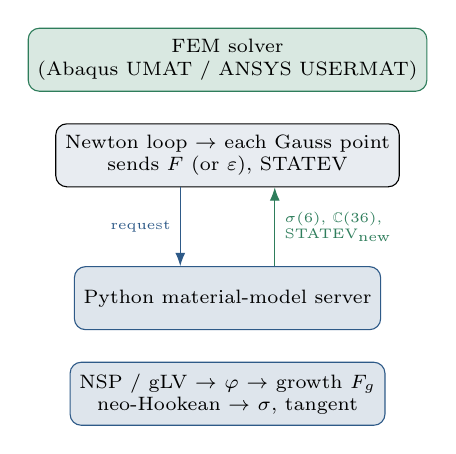
\begin{tikzpicture}[font=\scriptsize,node distance=5mm,
  box/.style={draw,rounded corners,minimum width=32mm,minimum height=8mm,align=center},
  fem/.style={box,fill=femgreen!18,draw=femgreen},
  py/.style={box,fill=pyblue!16,draw=pyblue}]
  \node[fem] (fem) {FEM solver\\ \scriptsize(Abaqus UMAT / ANSYS USERMAT)};
  \node[box,below=4mm of fem,fill=lgrey,minimum width=36mm] (gp) {Newton loop $\to$ each Gauss point\\ sends $F$ (or $\varepsilon$), STATEV};
  \node[py,below=10mm of gp,minimum width=36mm] (srv) {Python material-model server};
  \node[py,below=4mm of srv,minimum width=36mm] (model) {NSP / gLV $\to$ $\varphi$ $\to$ growth $F_g$\\ neo-Hookean $\to$ $\sigma$, tangent};
  % down: request
  \draw[-{Latex},pyblue] ($(gp.south)+(-6mm,0)$) -- node[left,font=\tiny]{request} ($(srv.north)+(-6mm,0)$);
  % up: response, routed on the right
  \draw[-{Latex},femgreen] ($(srv.north)+(6mm,0)$) -- node[right,font=\tiny,align=left]{$\sigma(6)$, $\mathbb{C}(36)$,\\STATEV$_{\text{new}}$} ($(gp.south)+(6mm,0)$);
\end{tikzpicture}
\\[0.3em]
{\scriptsize socket\,/\,wire round-trip per Gauss-point eval}
\end{column}
\begin{column}{0.46\textwidth}
\small
\textbf{Transport.} Self-contained Fortran UMAT does the TCP call via
\texttt{ISO\_C\_BINDING} to libc sockets — \textbf{no external object to link}
(sidesteps the \texttt{link\_sl} error). Host/port hard-wired \texttt{127.0.0.1:50007}.
\vspace{0.4em}

\textbf{Wire protocol} (Voigt 11,22,33,12,13,23; engineering shear):
{\scriptsize
\begin{align*}
\text{req:}&\ \ \text{NSTATV},\ \varepsilon(6),\ \Delta\varepsilon(6),\ \text{STATEV},\ E,\nu\\
\text{resp:}&\ \ \sigma(6),\ \mathbb{C}(36),\ \text{STATEV}_{\text{new}}
\end{align*}}

\textbf{Surrogate path.} Solve-time server is made \textbf{JAX-free}: the NSP
composition $\varphi_{\text{Pg}}(\text{step})$ is precomputed offline with JAX, the
per-Gauss-point server is pure-numpy neo-Hookean.
\end{column}
\end{columns}
\end{frame}

% ---------------------------------------------------------------- 4. The ladder
\begin{frame}{The verification ladder — de-risk one rung at a time}
\centering
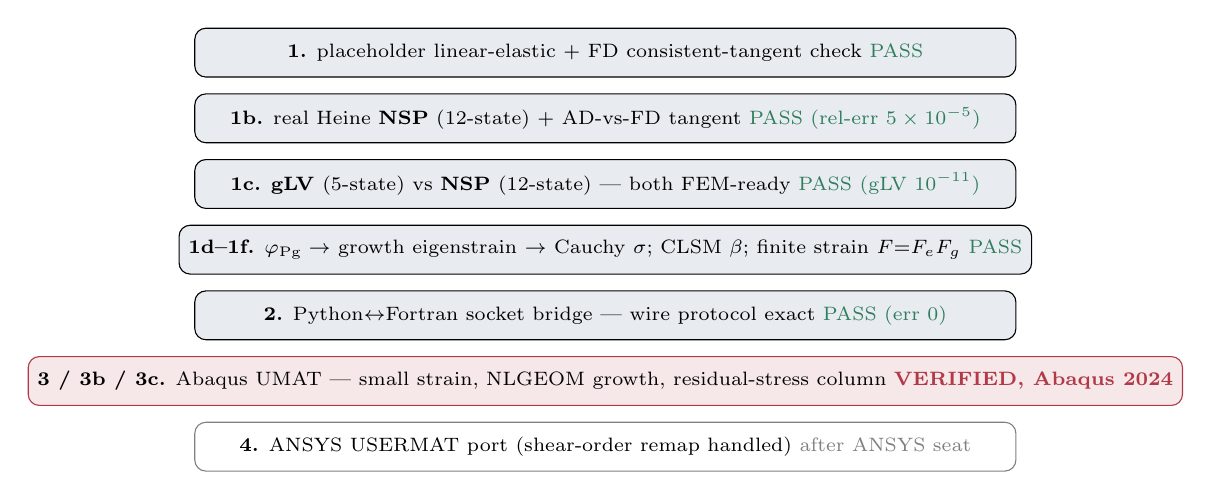
\begin{tikzpicture}[font=\scriptsize,
  rung/.style={draw,rounded corners,minimum width=0.86\textwidth,minimum height=6.2mm,align=left,fill=lgrey},
  ok/.style={accred}]
  \node[rung] (r1) {\textbf{1.} placeholder linear-elastic + FD consistent-tangent check \hfill \textcolor{femgreen}{PASS}};
  \node[rung,below=2.0mm of r1] (r1b) {\textbf{1b.} real Heine \textbf{NSP} (12-state) + AD-vs-FD tangent \hfill \textcolor{femgreen}{PASS (rel-err $5\times10^{-5}$)}};
  \node[rung,below=2.0mm of r1b] (r1c) {\textbf{1c.} \textbf{gLV} (5-state) vs \textbf{NSP} (12-state) — both FEM-ready \hfill \textcolor{femgreen}{PASS (gLV $10^{-11}$)}};
  \node[rung,below=2.0mm of r1c] (r1ef) {\textbf{1d--1f.} $\varphi_{\text{Pg}}\to$ growth eigenstrain $\to$ Cauchy $\sigma$; CLSM $\beta$; finite strain $F{=}F_e F_g$ \hfill \textcolor{femgreen}{PASS}};
  \node[rung,below=2.0mm of r1ef] (r2) {\textbf{2.} Python$\leftrightarrow$Fortran socket bridge — wire protocol exact \hfill \textcolor{femgreen}{PASS (err 0)}};
  \node[rung,below=2.0mm of r2,fill=accred!12,draw=accred] (r3) {\textbf{3 / 3b / 3c.} Abaqus UMAT — small strain, NLGEOM growth, residual-stress column \hfill \textcolor{accred}{\textbf{VERIFIED, Abaqus 2024}}};
  \node[rung,below=2.0mm of r3,fill=white,draw=gray] (r4) {\textbf{4.} ANSYS USERMAT port (shear-order remap handled) \hfill \textcolor{gray}{after ANSYS seat}};
\end{tikzpicture}
\vspace{0.3em}

\footnotesize Same Heine fit $(A,b)$, two constitutive laws — \emph{``same data, two models''} is a
clean thesis comparison axis. A consistent tangent is the prerequisite for the implicit FE Newton loop.
\end{frame}

% ---------------------------------------------------------------- 5. Verified on real Abaqus
\begin{frame}{Headline — verified on a real commercial solver (Abaqus 2024)}
\begin{columns}[T]
\begin{column}{0.5\textwidth}
\textbf{(a) Small-strain bridge.} \texttt{C3D8}, 1\% uniaxial strain, socket UMAT delivering the
Python model's stress per Gauss point:
\[
\sigma = [\,50.0,\,0,\,0,\dots],\quad \varepsilon=[\,0.01,\,{-}0.0045,\,{-}0.0045,\dots]
\]
i.e. exactly $\sigma_{xx}=E\,\varepsilon_{xx}$ and $\varepsilon_{\text{lat}}=-\nu\,\varepsilon_{xx}$.
\begin{block}{\small What this proves}
\footnotesize The Python$\leftrightarrow$FE coupling works on a \emph{commercial} solver, not just a mock.
\end{block}
\end{column}
\begin{column}{0.5\textwidth}
\textbf{(b) Finite-strain NSP growth.} NLGEOM job, multiplicative split $F=F_e F_g$, 20
increments all converged. Free-top element thickens in $z$:
\[
U_3(\text{top}) = 0.302 \approx \lambda_z-1,\qquad \sigma \approx 0
\]
(the free surface relieves $z$-only growth), with the NSP step counter
\textbf{SDV1 climbing $0\to20$} — one composition step per converged increment.
\vspace{0.4em}

\footnotesize Composition-driven finite-strain growth flows through the real solver per Gauss point;
the stress-free thickening matches the model's free-top prediction.
\end{column}
\end{columns}
\end{frame}

% ---------------------------------------------------------------- 6. CLSM-grounded calibration
\begin{frame}{Growth calibration grounded in CLSM data}
\begin{columns}[T]
\begin{column}{0.52\textwidth}
\small
Regress biofilm thickness (CLSM \texttt{zprofiles\_all\_ti.csv}) on the \textit{P. gingivalis} fraction:
\begin{itemize}
  \item \textbf{DH (dysbiotic): corr $0.88$, $\beta_{\text{depth}}\approx 17.2$} — thickness
        $22\to79$\,µm as $\varphi_{\text{Pg}}\!: 0.08\to0.21$.
  \item \textbf{CH (commensal control): opposite sign} — Pg drives thickening \emph{only} in dysbiosis.
\end{itemize}
\vspace{0.3em}
The flow-chamber lateral FOV is fixed $\Rightarrow$ growth is \textbf{anisotropic
(substratum-normal $z$)}: the eigenstrain lives in $zz$, not isotropic swelling.
\vspace{0.4em}

Calibrated $\varepsilon_{zz}$ reaches $\sim 1.2$--$2.4$ ($\lambda_z\!\sim\!2.4$): \textbf{finite strain}.
The additive small-strain split is invalid $\Rightarrow$ multiplicative
$F = F_e F_g,\ F_g=\mathrm{diag}(1,1,\lambda_z(\varphi_{\text{Pg}}))$.
\end{column}
\begin{column}{0.48\textwidth}
\centering
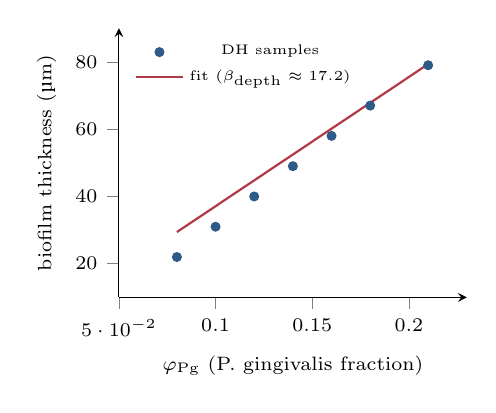
\begin{tikzpicture}
\begin{axis}[width=6.0cm,height=5.0cm,font=\scriptsize,
  xlabel={$\varphi_{\text{Pg}}$ (P. gingivalis fraction)},
  ylabel={biofilm thickness (µm)},
  xmin=0.05,xmax=0.23,ymin=10,ymax=90,
  axis lines=left,tick align=outside,
  legend style={font=\tiny,at={(0.02,0.98)},anchor=north west,draw=none}]
  % DH trend (corr 0.88)
  \addplot[only marks,mark=*,pyblue,mark size=1.6pt] coordinates {
    (0.08,22)(0.10,31)(0.12,40)(0.14,49)(0.16,58)(0.18,67)(0.21,79)};
  \addplot[accred,thick,domain=0.08:0.21,samples=2] {-1.3 + 384*x};
  \legend{DH samples, fit ($\beta_{\text{depth}}\approx17.2$)}
\end{axis}
\end{tikzpicture}
\\[-0.2em]
\footnotesize\textit{DH: thickness tracks $\varphi_{\text{Pg}}$, corr $0.88$.}
\end{column}
\end{columns}
\end{frame}

% ---------------------------------------------------------------- 7. The FEM-only result
\begin{frame}{Headline — the FEM-only result: differential-growth residual stress}
\begin{columns}[T]
\begin{column}{0.5\textwidth}
\small
Multi-element growth \textbf{column}, depth-graded growth from the CLSM $\varphi_{\text{Pg}}(z)$
profile, \textbf{laterally confined}, free top. The in-plane residual stress $S_{11}(z)$ tracks
$\varphi_{\text{Pg}}(z)$:
\[
S_{11}\!:\ -136\ (\text{Pg-poor mid})\ \longrightarrow\ -354\ (\text{Pg-rich top}),
\]
\[
S_{33}\approx 0\quad(\text{free top}).
\]
\begin{block}{\small Why this needs the FEM}
\footnotesize A single element cannot produce this. \textbf{Meaningful residual / delamination stress
needs a spatial growth gradient} — exactly the multi-element job. \emph{This is the thesis.}
Verified on Abaqus 2024.
\end{block}
\end{column}
\begin{column}{0.5\textwidth}
\centering
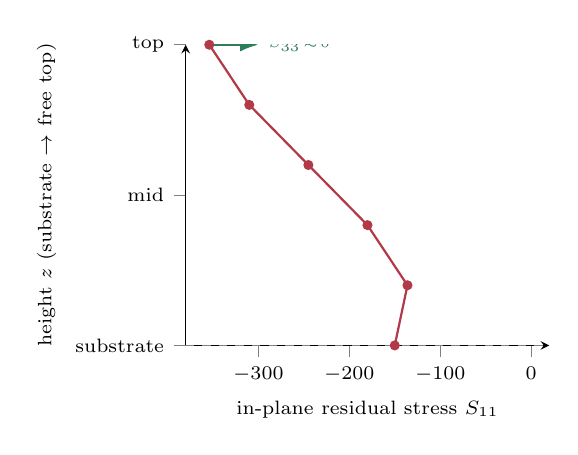
\begin{tikzpicture}
\begin{axis}[width=6.2cm,height=5.4cm,font=\scriptsize,
  xlabel={in-plane residual stress $S_{11}$},
  ylabel={height $z$ (substrate $\to$ free top)},
  xmin=-380,xmax=20,ymin=0,ymax=1,
  axis lines=left,tick align=outside,
  ytick={0,0.5,1},yticklabels={substrate,mid,top}]
  \addplot[accred,thick,mark=*,mark size=1.4pt] coordinates {
    (-150,0.00)(-136,0.20)(-180,0.40)(-245,0.60)(-310,0.80)(-354,1.00)};
  \addplot[gray,dashed,domain=-380:20,samples=2] {0}; % visual S33~0 not shown
  \draw[femgreen,thick,-{Latex}] (axis cs:-354,1.0) -- (axis cs:-300,1.0)
       node[right,font=\tiny,femgreen]{$S_{33}\!\approx\!0$};
\end{axis}
\end{tikzpicture}
\\[-0.2em]
\footnotesize\textit{Compressive in-plane stress, deepest where $\varphi_{\text{Pg}}$ is highest (top).}
\end{column}
\end{columns}
\end{frame}

% ---------------------------------------------------------------- 8. Method polish
\begin{frame}{Method polish — consistent tangent and growth modes}
\begin{columns}[T]
\begin{column}{0.55\textwidth}
\textbf{Consistent neo-Hookean Jaumann tangent.} Replaces the approximate elastic Jacobian in both
finite-strain servers — the production tangent for the implicit Newton loop:
\[
\lambda' = \frac{\lambda}{J},\qquad \mu' = \frac{\mu-\lambda\ln J}{J}.
\]
It reduces \emph{exactly} to the elastic tangent at $F_e=I$ (verified).
\vspace{0.5em}

\textbf{Confinement cost.} Fully confined $140\%$ growth costs $\sim 15$--$20\,\mu$ in both
formulations — but only $F=F_e F_g$ is kinematically valid at $\lambda_z\!\sim\!2.4$.
\end{column}
\begin{column}{0.45\textwidth}
\textbf{Two growth modes} (selectable):
\begin{itemize}
  \item \texttt{depth} (default) — anisotropic, substratum-normal; eigenstrain in $zz$.
    CLSM-grounded.
  \item \texttt{iso} — volumetric swelling; comparison variant $\to$ in-plane residual stress.
\end{itemize}
\vspace{0.5em}
\footnotesize The realistic free-top BC is $\approx$ stress-free (biofilms thicken without failure);
residual stress arises from the \emph{spatial gradient}, not the magnitude.
\end{column}
\end{columns}
\end{frame}

% ---------------------------------------------------------------- 9. Abaqus -> ANSYS mapping
\begin{frame}{From Abaqus UMAT to ANSYS USERMAT — a near-copy}
\centering
\renewcommand{\arraystretch}{1.2}
\small
\begin{tabular}{l l l}
\hline
\textbf{Abaqus UMAT} & \textbf{ANSYS USERMAT} & \textbf{note}\\
\hline
\texttt{STRESS} & \texttt{stress} & Cauchy, same Voigt order\\
\texttt{DDSDDE} & \texttt{dsdePl} & consistent tangent $6\times6$\\
\texttt{STATEV} / \texttt{*DEPVAR} & \texttt{ustatev} / \texttt{TB,STATE} & state variables\\
\texttt{PROPS} / \texttt{*USER MATERIAL} & \texttt{prop} / \texttt{TB,USER} & material constants\\
\texttt{DSTRAN},\,\texttt{STRAN} & \texttt{dStrain},\,\texttt{Strain} & engineering shear both\\
\texttt{abaqus ... user=umat.f} & \texttt{ANSUSERMAT} + \texttt{/UPF} & same C socket shim reused\\
\hline
\end{tabular}
\vspace{0.6em}

\footnotesize The wire protocol and Voigt convention are shared, so rung 3 $\to$ 4 is a near-copy;
the only substantive difference is a \textbf{shear-order remap}, handled in the USERMAT skeleton.
\end{frame}

% ---------------------------------------------------------------- 10. Roadmap
\begin{frame}{Roadmap / outlook}
\begin{enumerate}
  \item \textbf{ANSYS USERMAT port} — after an IKM/LUH license seat; match Felix's ANSYS version for
    ABI. The proven bridge makes this a near-copy (shear-order remap handled).
  \item \textbf{Verification} — mesh convergence of the residual-stress column; tangent vs FD across
    the mesh.
  \item \textbf{Validation} — reference cases against the current phenomenological law; 2--3 standard
    benchmarks with Felix.
  \item \textbf{Biofilm-specific constitutive law} — $\mu$ from biofilm rheology; buckling /
    delamination on multi-element meshes.
  \item \textbf{Clinical interpretation} — residual stress $\to$ detachment / peri-implantitis risk
    (the NIFE through-line).
\end{enumerate}
\vspace{0.3em}
\footnotesize Open: Junker + Soleimani must agree on \emph{one} title before Page 1 to the
Prüfungsamt; Felix handover meeting + acknowledgement of his PhD FEM contribution.
\end{frame}

% ---------------------------------------------------------------- 11. Take-home
\begin{frame}{Take-home}
\begin{enumerate}
  \item The Python$\leftrightarrow$FE coupling is \textbf{proven on a real solver}
    (Abaqus 2024): small-strain $\sigma_{xx}=E\varepsilon$ and finite-strain NSP growth
    ($U_3\to\lambda_z-1$, $\sigma\approx0$, SDV1 $0\to20$).
  \item \textbf{Two constitutive laws are FEM-ready} from the same Heine fit — gLV (5-state) and
    NSP (12-state), each with a consistent tangent.
  \item Growth is \textbf{calibrated on real CLSM data} (DH corr $0.88$, $\beta_{\text{depth}}\approx17.2$)
    and is \textbf{finite strain} ($\lambda_z\!\sim\!2.4$) $\Rightarrow$ multiplicative $F=F_e F_g$.
  \item The \textbf{FEM-only result}: depth-graded growth $\to$ residual stress profile
    $S_{11}(z)$ from $-136$ to $-354$, tracking $\varphi_{\text{Pg}}(z)$ — the differential-growth
    stress a single element cannot produce.
\end{enumerate}
\vspace{0.5em}
\centering\textit{Proven on Abaqus, FEM-ready constitutive laws, CLSM-calibrated growth —
ready to port to ANSYS.}
\end{frame}

\end{document}
